  A comprehensive study in the Hudson Bay region of the Canadian Shield [Thomson et. al., 2010] employs data from 35 stations, of which, 27 stations share an error acceptable for comparison in both datasets. There is strong correlation, 0.97, between crustal thickness values (Fig \ref{fig:thompsonCompH}). The velocity ratio data has a lower correlation of 0.49 (Fig \ref{fig:thompsonCompR}) and a mean difference of 0.02. As indicated in section \ref{section:VpVsMethod} there is less resolution in $R$ so the lower correlation for this parameter is not unexpected.

 Another study conducted in the Grenville Orogen [Eaton et al., 2006] utilizes data from 29 stations, with two stations being excluded due to low quality and high error. Again, there is strong correlation in $H$, 0.89, and lower correlation in $R$, 0.56 (Figs \ref{fig:eatonCompH}, \ref{fig:eatonCompR}). The mean difference in $R$ between the two datasets is 0.04.

\begin{figure}
  \centering
    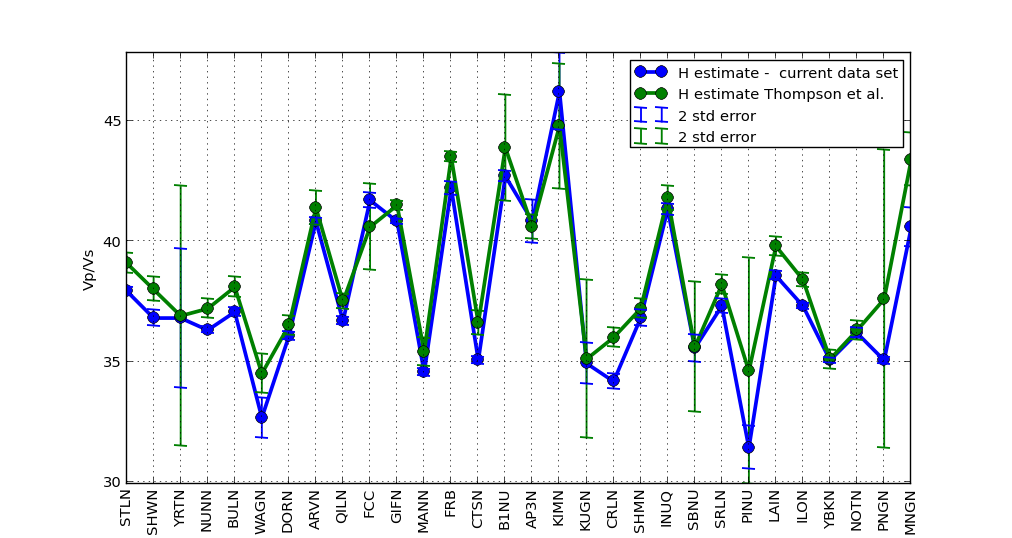
\includegraphics[width=\textwidth]{thompsonComparisonH}
  \caption{Comparison of crustal thickness $H$ data from this study with data from Thompson et. al. (2010). Data shows a Pearson correlation of 0.95}
  \label{fig:thompsonCompH}
\end{figure}

\begin{figure}
  \centering
    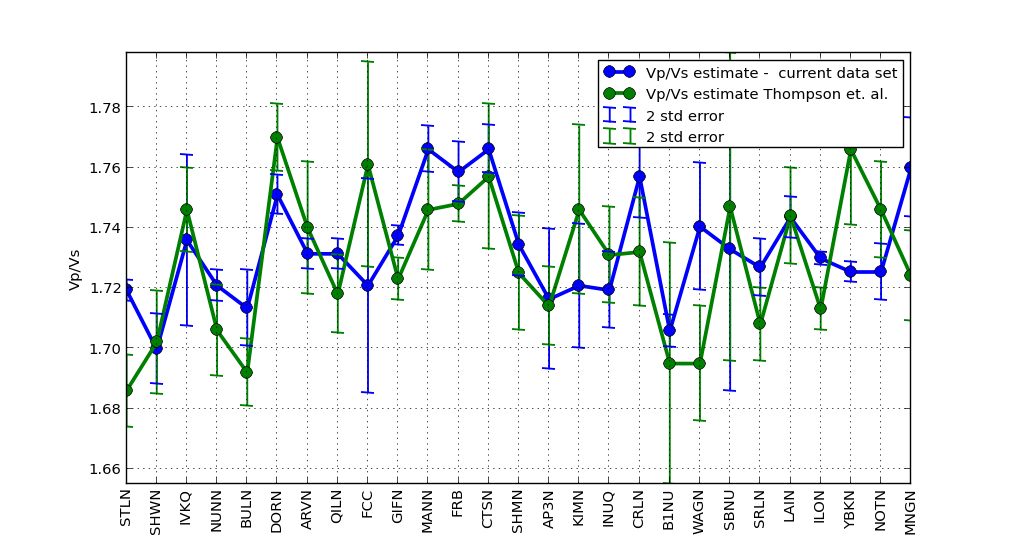
\includegraphics[width=\textwidth]{thompsonComparisonR}
  \caption{Comparison of $V_P / V_R$ data from this study with data from Thomspson et. al. (2010). Data shows a Pearson correlation of 0.5}
  \label{fig:thompsonCompR}
\end{figure}

\begin{figure}
  \centering
    \includegraphics[width=\textwidth]{eatonComparisonH}
  \caption{Comparison of crustal thickness $H$ data from this study with from Eaton et. al. (2010). Data shows a Pearson correlation of 0.95}
  \label{fig:eatonCompH}
\end{figure}

\begin{figure}
  \centering
  \includegraphics[width=\textwidth]{eatonComparisonR}
  \caption{Comparison of $V_P / V_R$ data from this study with data from Eaton et. al. (2010). Data shows a Pearson correlation of 0.5}
  \label{fig:eatonCompR}
\end{figure}

\begin{figure}
  \centering
  \includegraphics[width=\textwidth]{darbyshireComparisonH}
  \caption{Comparison of crustal thickness $H$ data from this study with data from Darbyshire et. al. (2010). Data shows a Pearson correlation of 0.95}
  \label{fig:darbyshireCompH}
\end{figure}

\begin{figure}
  \centering
  \includegraphics[width=\textwidth]{darbyshireComparisonR}
  \caption{Comparison of $V_P / V_R$ data from this study with data from Darbyshire et. al. (2010). Data shows a Pearson correlation of 0.5}
  \label{fig:darbyshireCompR}
\end{figure}
